%=======================================================================================================================
\clearpage
\subsection{Miura scheme}
\label{sub:miura}
%=======================================================================================================================
%
No artificial diffusion term is needed for the scalar quantities because the advection of $\density{}{}{}$ and $\vpotemp{}{}{}$ is discretized with an upwind-biased second-order accurate scheme following \cite{miuraUpwindBiasedConservativeAdvection2007}.

\begin{align}
  &\density{\n}{\e}{\k} = \densityref{\e}{\k} + \densityprime{\n}{\c 0/1}{\k} + \Delta^{\hat{x}}_{\c - \text{btrj}} \densityprimedx{\n}{\c}{\k} + \Delta^{\hat{y}}_{\c - \text{btrj}} \densityprimedy{\n}{\c}{\k} \\
  &\vpotemp{\n}{\e}{\k} = \vpotempref{\e}{\k} + \vpotempprime{\n}{\c 0/1}{\k} + \Delta^{\hat{x}}_{\c - \text{btrj}} \vpotempprimedx{\n}{\c}{\k} + \Delta^{\hat{y}}_{\c - \text{btrj}} \vpotempprimedy{\n}{\c}{\k}
\end{align}

\begin{align}
  & \densityprimedx{\n}{\c}{\k} = \sum_{\offProv{c2e2co}} \geofacgrgx\ \densityprime{\n}{\c}{\k} \\
  & \densityprimedy{\n}{\c}{\k} = \sum_{\offProv{c2e2co}} \geofacgrgy\ \densityprime{\n}{\c}{\k} \\
  & \vpotempprimedx{\n}{\c}{\k} = \sum_{\offProv{c2e2co}} \geofacgrgx\ \vpotempprime{\n}{\c}{\k} \\
  & \vpotempprimedy{\n}{\c}{\k} = \sum_{\offProv{c2e2co}} \geofacgrgy\ \vpotempprime{\n}{\c}{\k}
\end{align}

The \ibm\ (\IBM) handles these operations by zeroing the gradient computation in cells adiacent to masked cells---those indicated with a dotted pattern in figure~\ref{fig:miura}.
This reduces the order of the scheme from second to first for those edge points that pick upwind values in dotted cells.


\begin{figure}[h!]
  \begin{center}
    \includesvg[height=150pt]{imgs/miura} \hspace{10pt}
    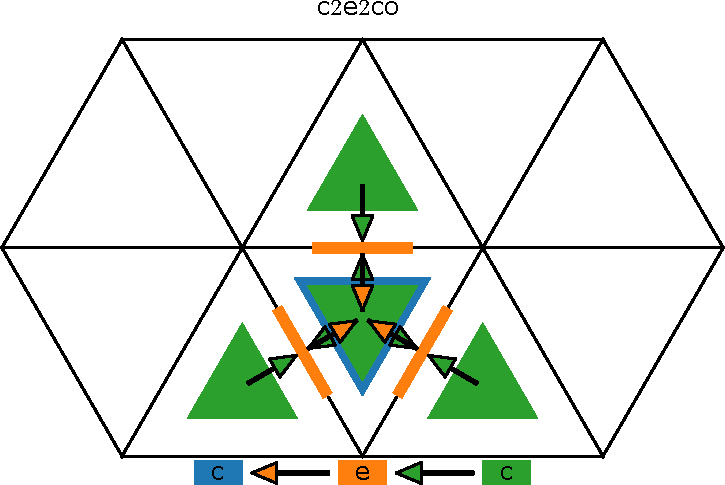
\includegraphics[height=150pt]{imgs/offsetProvider_c2e2co} \hspace{10pt}
    \includesvg[height=150pt]{imgs/masked_cells_01}
  \end{center}
  \caption{Miura scheme definition and offset provider used for the horizontal derivative computations}
  \label{fig:miura}
\end{figure}

